\section*{Research Methodology}

The research methodology for developing and evaluating the proposed LLM-guided data augmentation framework for few-shot action recognition is structured into distinct phases, each addressing a specific aspect of the framework. These phases are designed to progressively build and refine the system, culminating in a rigorous evaluation of its performance and effectiveness.


\subsection*{Phase 1: LLM-Based Action Description Generation}
This initial phase focuses on harnessing the capabilities of Large Language Models (LLMs) to generate comprehensive and diverse descriptions of human actions. A pre-trained LLM, such as GPT-3 or an equivalent open-source alternative, will be utilized as the foundation. The core of this phase involves fine-tuning the selected LLM on a curated dataset of action descriptions. This dataset will be a combination of existing video captioning datasets and manually curated descriptions tailored to the specific actions of interest. Prompt engineering is crucial to elicit the desired variations, counterfactual scenarios, and subtle nuances in action execution. We will explore different prompting strategies, including zero-shot prompting (where the LLM generates descriptions without any examples), few-shot prompting (where the LLM is provided with a few examples of action descriptions), and fine-tuning with specifically designed prompts that encourage the generation of diverse and semantically rich outputs. The quality of the generated descriptions will be assessed through a combination of human evaluation, where human annotators rate the relevance and accuracy of the descriptions, and automated metrics, such as BLEU or METEOR, which measure the semantic similarity between the generated descriptions and ground truth descriptions.

\subsection*{Phase 2: Augmentation Parameter Mapping}
his phase bridges the gap between the textual descriptions generated by the LLM and the concrete parameters required to perform data augmentation. A mapping model will be developed to translate the LLM-generated descriptions into a set of parameters for different augmentation techniques. This model will take the textual description as input and output a vector of parameters that control aspects such as the degree of rotation, the size of the crop, the intensity of color jittering, and the temporal displacement. Different architectures for this mapping model will be explored, including recurrent neural networks (RNNs), which are well-suited for processing sequential data like text, and transformers, which have demonstrated superior performance in capturing long-range dependencies in language. The mapping model will be trained on a dataset of paired descriptions and corresponding augmentation parameters. This dataset will be generated through a combination of manual annotation, where human annotators manually associate descriptions with specific parameter values, and programmatic generation, where rules based on keywords or phrases in the descriptions are used to automatically generate parameter values. The quality of the mapping will be evaluated by assessing the realism and diversity of the resulting augmented samples. Perceptual similarity metrics will be employed to quantify the similarity between the augmented samples and real video data.

\subsection*{Phase 3: Data Augmentation and Action Recognition Training}
he generated augmentation parameters will be used to apply transformations to the limited training examples in the few-shot setting. A variety of augmentation techniques will be utilized, including standard transformations such as cropping, rotation, flipping, and jittering (color, temporal), as well as advanced techniques such as Mixup and CutMix, adapted for video data. The possibility of using GANs or diffusion models conditioned on the LLM descriptions to generate entirely new synthetic video segments will also be explored. For few-shot action recognition, a meta-learning approach, specifically MAML, will be employed. The model architecture will be based on a convolutional neural network (CNN) designed for video processing, such as a 3D-CNN or a two-stream network. The model will be trained on the augmented dataset using standard optimization algorithms like Adam. Performance will be evaluated using the N-way K-shot accuracy metric, as well as precision, recall, and F1-score, to provide a comprehensive assessment of the model's ability to generalize from limited examples.

% % \begin{center}
% %     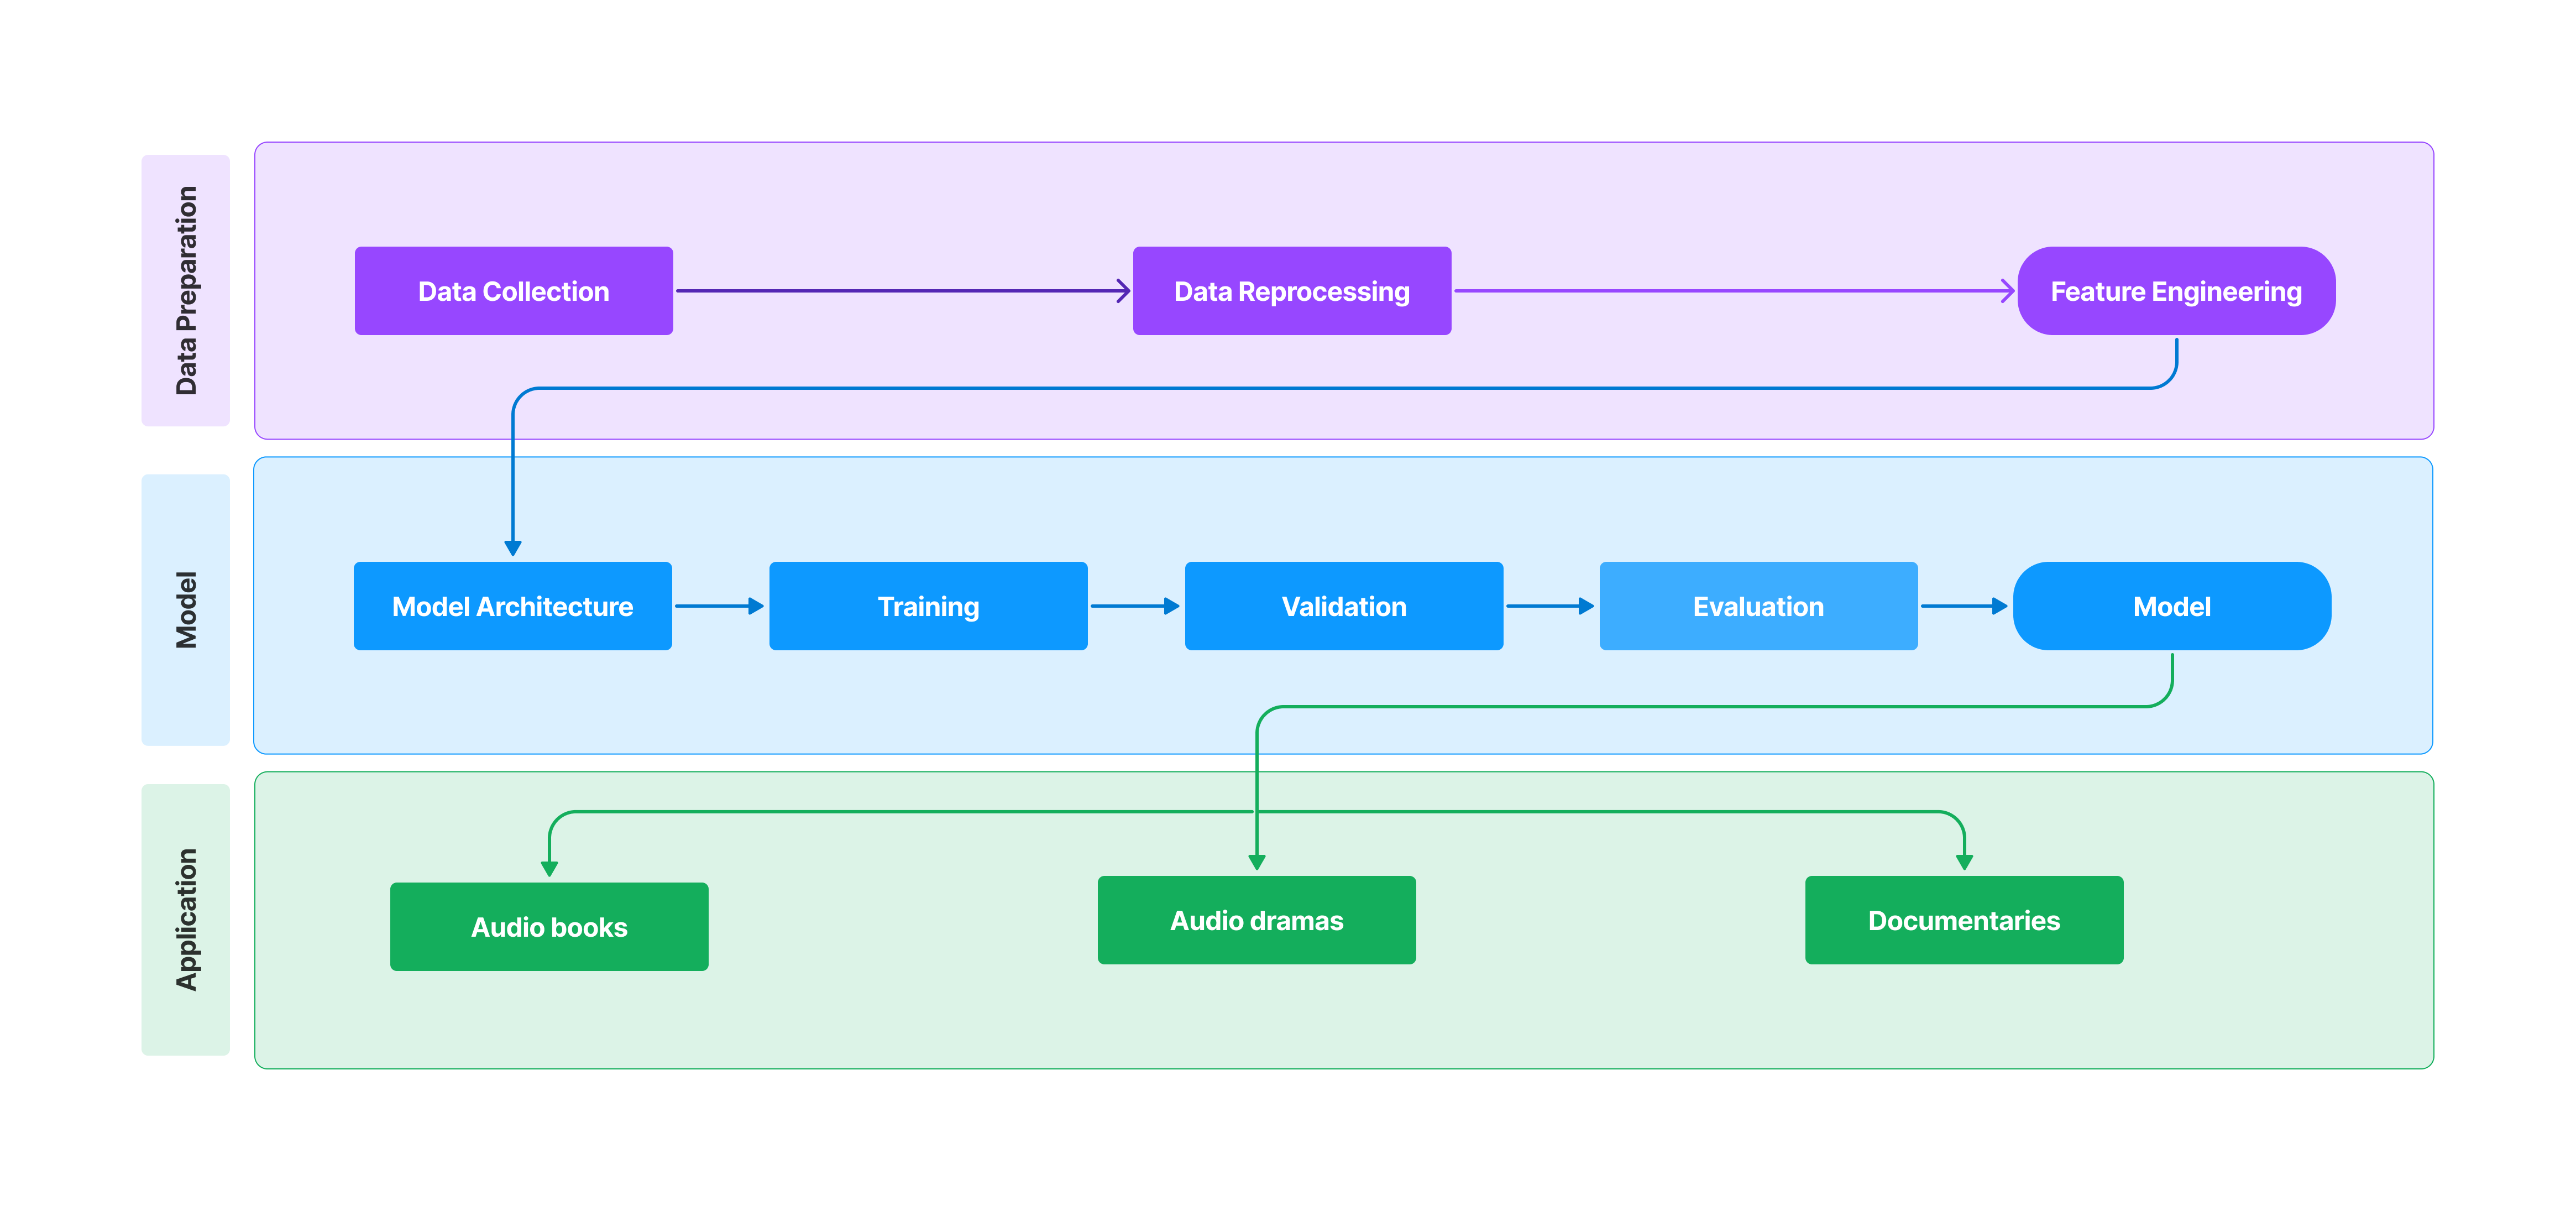
\includegraphics[width=1.0\textwidth]{image.png}
% %     \captionof{figure}{Research flow}
% % \end{center}